\documentclass[a4paper,natbib,man]{apa6}
%\documentclass[a4paper,man,natbib,floatsintext]{apa6}
%The APA6 class: http://ctan.math.utah.edu/ctan/tex-archive/macros/latex/contrib/apa6/apa6.pdf

\usepackage[english]{babel}
\usepackage[utf8x]{inputenc}
\usepackage{amsmath}
\usepackage{graphicx}
\usepackage[colorinlistoftodos]{todonotes}
\def\citeA{\citep}


% Words in text: 3309
% Words in appendices: ~700

%% User-specific lines 
\usepackage{amsmath,amssymb,amsthm}
\usepackage{soul}

%\newtheorem{thm}{Theorem}
%\newtheorem{lem}{Lemma}
%\newtheorem{dfn}{Definition}

\usepackage{amssymb,amsfonts,amsmath,amsthm}
\usepackage{mathrsfs}
\usepackage{array}
\usepackage{lineno}
\usepackage{color}
%\usepackage{ulem}

%\linenumbers

%% Macro
\def\diam{\mathrm{diam}}
\newcommand{\floor}[1]{\lfloor #1 \rfloor}
\newcommand{\ceil}[1]{\lceil #1 \rceil}
\newcommand{\one}[1]{\mathbf{1}_{#1}}
\newcommand{\vctr}[1]{\mathrm{vec}\left( #1 \right)}
\newcommand{\diag}[1]{\mathrm{diag}\left( #1 \right)}
%\newcommand{\Diag}[1]{\mathrm{Diag}\left( #1 \right)}
\newcommand{\Diag}[1]{\mathrm{Dg}\left( #1 \right)}
\newcommand{\learninggame}{learning-and-game }
\def\hsymb#1{\mbox{\strut\rlap{\smash{\Huge$#1$}}\quad}}
\newcommand{\VecSet}[2]{\mathbb{#1}^{#2}}
\newcommand{\MatSet}[2]{\mathbb{#1}^{{#2}\times{#2}}}
\newcommand{\MatSets}[3]{\mathbb{#1}^{{#2}\times{#3}}}
\newcommand{\Encode}[2]{\mathcal{C}_{#1,#2}}
\newcommand{\Simplex}[1]{\mathbb{S}^{#1}}
\newcommand{\SimMat}[1]{\mathbb{S}^{#1 \times #1}}
\newcommand{\SimMats}[2]{\mathbb{S}^{#1 \times #2}}

\newcommand{\Trans}[2]{#1^{(#2)}}
\newcommand{\TransBlock}[3]{#1_{#3}^{(#2)}}
%\newcommand{\TransBlockVec}[4]{#1_{#3, #4}^{(#2)}}
\newcommand{\TransBlockVec}[4]{#1_{N(#3-1) + #4}^{(#2)}}

\newcommand{\TransBlockNo}[2]{#1_{#2}}
\newcommand{\TransBlockVecNo}[3]{#1_{#2, #3}}
\newcommand{\zero}[1]{\mathbf{0}_{#1}}
\newcommand{\rank}[1]{\text{rank}\left(#1\right)}

%% For the application
\newcommand{\dd}[0]{\text{d}}

%\newcommand{\argmax}{\mathop{\rm arg~max}\limits}
%\newcommand{\argmin}{\mathop{\rm arg~min}\limits}
\DeclareMathOperator*{\argmin}{arg\,min} %argmin
\DeclareMathOperator*{\argmax}{arg\,max} %argmax


%\newtheorem{thm}{Theorem}[section]
\newtheorem{thm}{Theorem}[]
%\newtheorem{cor}[thm]{Corollary}
\newtheorem{prop}{Proposition}
%\newtheorem{lem}[thm]{Lemma}
\newtheorem{lem}[]{Lemma}
%\newtheorem{def}[thm]{Definition}
\newtheorem{definition}[]{Definition}
\newtheorem{cor}[]{Corollary}

%\newcommand{\SH}[1]{\textcolor{red}{#1}}
%\newcommand{\GK}[1]{\textcolor{orange}{#1}}
\newcommand{\SH}[1]{#1}
\newcommand{\GK}[1]{#1}

\title{Active learners can learn what simple samplers cannot: A Zipf-distributed vocabulary from limited data} 
%\title{A theoretical analysis of active cross-situational word learning under Zipfian distributions}
\shorttitle{Active word learning}
%\author{Shohei Hidaka$^1$, Takuma Torii$^1$, and George Kachergis$^2$}
\author{Anonymous author(s)}
%\affiliation{$^1$Japan Advanced Institute for Science and Technology and $^2$Stanford University}
\affiliation{}

% Brief articles reporting original empirical findings, major theoretical advances or crucial developments that warrant rapid communication to the scientific community - limit 3000 words including abstract (excluding references)
% http://app.uio.no/ifi/texcount/online.php  2940 words as of 9/11/18 (+122 in captions)

% abstract is 186 words 9/11/18
\abstract{
Children learn thousands of words in the first several years of life, inspiring many theoretical and empirical studies seeking to understand the speed of word learning. The present study revisits recent theoretical analyses of simple sampling models with uniformly-distributed word frequency, and considers a more realistic Zipfian (i.e., power-law) distribution of words and referents. 
Our new mathematical analysis finds that simple sampling models are unable to account for word learning in feasible time under Zipf-distributed word and referent frequencies. To salvage learning under realistic distributional assumptions, we propose an active learning model which assumes that learners and/or caregivers select (or construct) the contexts from which words are sampled. Using simulations and mathematical analysis, we show that active learners choosing optimal learning situations learn hundreds of times faster than passive learners faced with randomly-sampled situations. Thus, as suggested by past empirical studies, we find theoretical support for the idea that statistical structure in real-world situations--potentially created by the self-directed learner or beneficent teachers--is a potential remedy for the difficulty of learning a Zipf-distributed vocabulary.}

\begin{document}
\maketitle

\section{The remarkable pace of word learning}

Language acquisition proceeds quickly in young children, who within their first year learn the sounds of their language \citep{Kuhl:1992}, begin segmenting speech \citep{Saffran:1996} and even produce their first words \citep{Hulit:2002}.
By 18 months, children can produce on average 50 words and comprehend 100-150 \citep{Hulit:2002}, with vocabulary size growing to around 1,000 words by age 3 \citep{Hart:1995}, and reaching roughly 60,000 words by 18 years of age \citep{Bloom:2000}.
Under the assumption that each child has 8 hours of word learning opportunity every day, these estimates have the child learning a new word every learning hour for 18 years, on average. 
This pace seems remarkable, given the storied complexity of the learning environment: a given word could refer to any of infinite possible meanings in any given situation \citep[cf.][]{Blythe:2016}. % introduce Smith & Yu's short arm / single object finding at some point
\GK{Although older learners no doubt accelerate word learning as they begin to read, children already show an accelerating pace of learning in the second year of life, growing from an average of 11 words at 12 months to over 300 words by 24 months \citep{wordbankbook,fenson2007}.
How might young children tackle the daunting problem of mapping words to referents?}


A variety of heuristics and mechanisms are thought to help learners mitigate referential uncertainty, and empirical studies have shown that young children can take advantage of many of them in the laboratory. 
For example, children can leverage social cues \citep{HirshPasek:2000}, can learn a word from a single informative instance \citep[i.e., {\em fast-map};][]{Carey:1978,Spiegel:2011}, tend to assume words refer to whole objects \citep{Macnamara:1972}, \GK{and are biased to form mutually exclusive word-referent mappings \citep{Merriman:1989}}. 
These heuristics are assumed to aid the process of {\it cross-situational learning}: acquiring words by accumulating evidence for meanings across multiple contexts--an ability demonstrated in the lab by infants and adults \citep{Smith:2008vg,Yu:2007}. 
However, determining the relative contributions of these myriad heuristics to naturalistic cross-situational word learning remains a challenge, \GK{despite their inclusion in various computational models of word learning, both because such models are primarily applied to experimental settings, and because the complexity and structure of real-world learning environments is largely unknown \citep[though see][]{Smith:2018,Suanda:2018,Clerkin:2017}.}

\GK{Moreover, there is disagreement over the basic mechanisms governing word learning: hypothesis-testing models view the problem as one of inference in which the learner may propose and test a single mapping for each word and referent \citep[e.g.,][]{Trueswell:2013}, while associative models gradually accumulate noisy knowledge traces representing graded links between multiple words and referents \citep[e.g.,][]{McMurray:2012,Kachergis:2012gi}.
Both types of models can implement fast mapping, mutual exclusivity, and other heuristics, and although they are not always equivalent, it has been shown that these models may often mimic one another's behavior \citep{Yu:2012hyp}, making it difficult to choose a general approach to modeling word learning. 
Nonetheless, it has proven useful to test the overall strength of simple learning mechanisms in idealized simulations of the language learning environment in order to explore the long-term behavior and plausibility of such mechanisms for learning an adult-sized (60,000-word) vocabulary \citep{Blythe:2010,Vogt:2012,Blythe:2016}.}


As a starting point, we build on these mathematical analyses, which model word learning as a random sampling process of a single word, a target meaning, and several distractor meanings in each situation. 
\cite{Blythe:2010,Blythe:2016} analyzed an idealized learning model that learns each word on its first sample (i.e., {\it fast-mapping}, or one-shot learning), in order to estimate the fastest possible learning rate needed to learn a full-sized vocabulary.
Under the simplifying assumptions that each word is independently learned via fast-mapping, and that word frequency (WF) is uniformly-distributed (Figure~\ref{fig-overview}, top left), their mathematical analysis of the model showed that a cross-situational learner is likely to learn an adult-sized vocabulary (i.e., $\sim60,000$) words after only $\sim940,000$ samples, a number of spoken words that is well within the bounds of human life experience, requiring roughly 142 learning instances per day for 18 years \citep{Blythe:2010}. %
Blythe \textit{et al}.'s analytical estimate has been treated as a theoretical implication that learning via independent fast-mapping of words is sufficiently powerful to be a model of child word learning. 
\cite{Blythe:2010} also considered a Zipf-distributed target word distribution, finding that it should be slower by a factor that depends on the size of the to-be-learned vocabulary (11.58 for 60,000 words, so 10.9 million). % 940000*11.58 = 10,885,200;  -- Blythe et al. 2010's upper bound based on Hart and Risley (2003): 2,100 words per hour, 14 h of exposure per day for 18 years = 2100 * 14 * 365 * 18 = 193,158,000
% realistic bound: 1000 * 14 * 365 * 18 = 91,980,000

However, that analysis did not consider nonuniform referent distributions, which might be expected if meaning distribution is usage-based. 
Indeed, analysis of egocentric views from head-mounted cameras on 8- to 10-month-old infants shows a right-skewed frequency distribution of referents \citep{Clerkin:2017}, suggesting a Zipfian distribution of referents in naturalistic developmental learning environments. 
\cite{Vogt:2012} explored the effects of Zipf-distributed words and incidental meanings via Monte Carlo simulation using a model framework similar to that of \cite{Blythe:2010}, and found that learning times increase super-exponentially as a function of the ratio of the context size ($C$) to the number of incidental meanings ($M$). 
Learning on human-scale timelines were only possible for ratios of $C/M \leq .1$, meaning that in any given learning situation less than a tenth of the possible meanings should be plausible. 



\subsection{The present study}

The present study reinspects independent fast-mapping under a more realistic power-law word frequency distribution (WFD) that is characteristic of natural language \citep{Zipf:1949}. 
Our new mathematical analysis implies that the learning rate of independent fast mapping is quite sensitive to nonuniform distributions of words and referents. 
Critically, under a Zipfian word and referent frequency distribution, even fast-mapping--the most efficient learning--is typically too slow to learn 60,000 words in 18 years. 
Intuitively, the difficulty with quickly learning a long-tailed distribution under random sampling is that a learner must wait a very long time to hear the large proportion of low-frequency words.
We show that independent fast-mapping cannot account for children's rate of word learning in any distribution where a significant portion of words are infrequently sampled. 
We confirm that simulated learning from the Zipfian WFD in the CHILDES database \citep{MacWhinney1990}, a corpus of child-directed speech, is quite slow.

% Vogt:2012 / Blythe:2010 model assumptions (as Vogt wrote): (a) a word is always exposed in a situation where its meaning is present, (b) each word and situation are perceived without errors, (c) all situations have the same number of distinct incidental meanings, (d) all meanings are given, so there is no need for categorization, and (e) the lexicon is unambiguous.

\begin{figure}[h]
\begin{center}
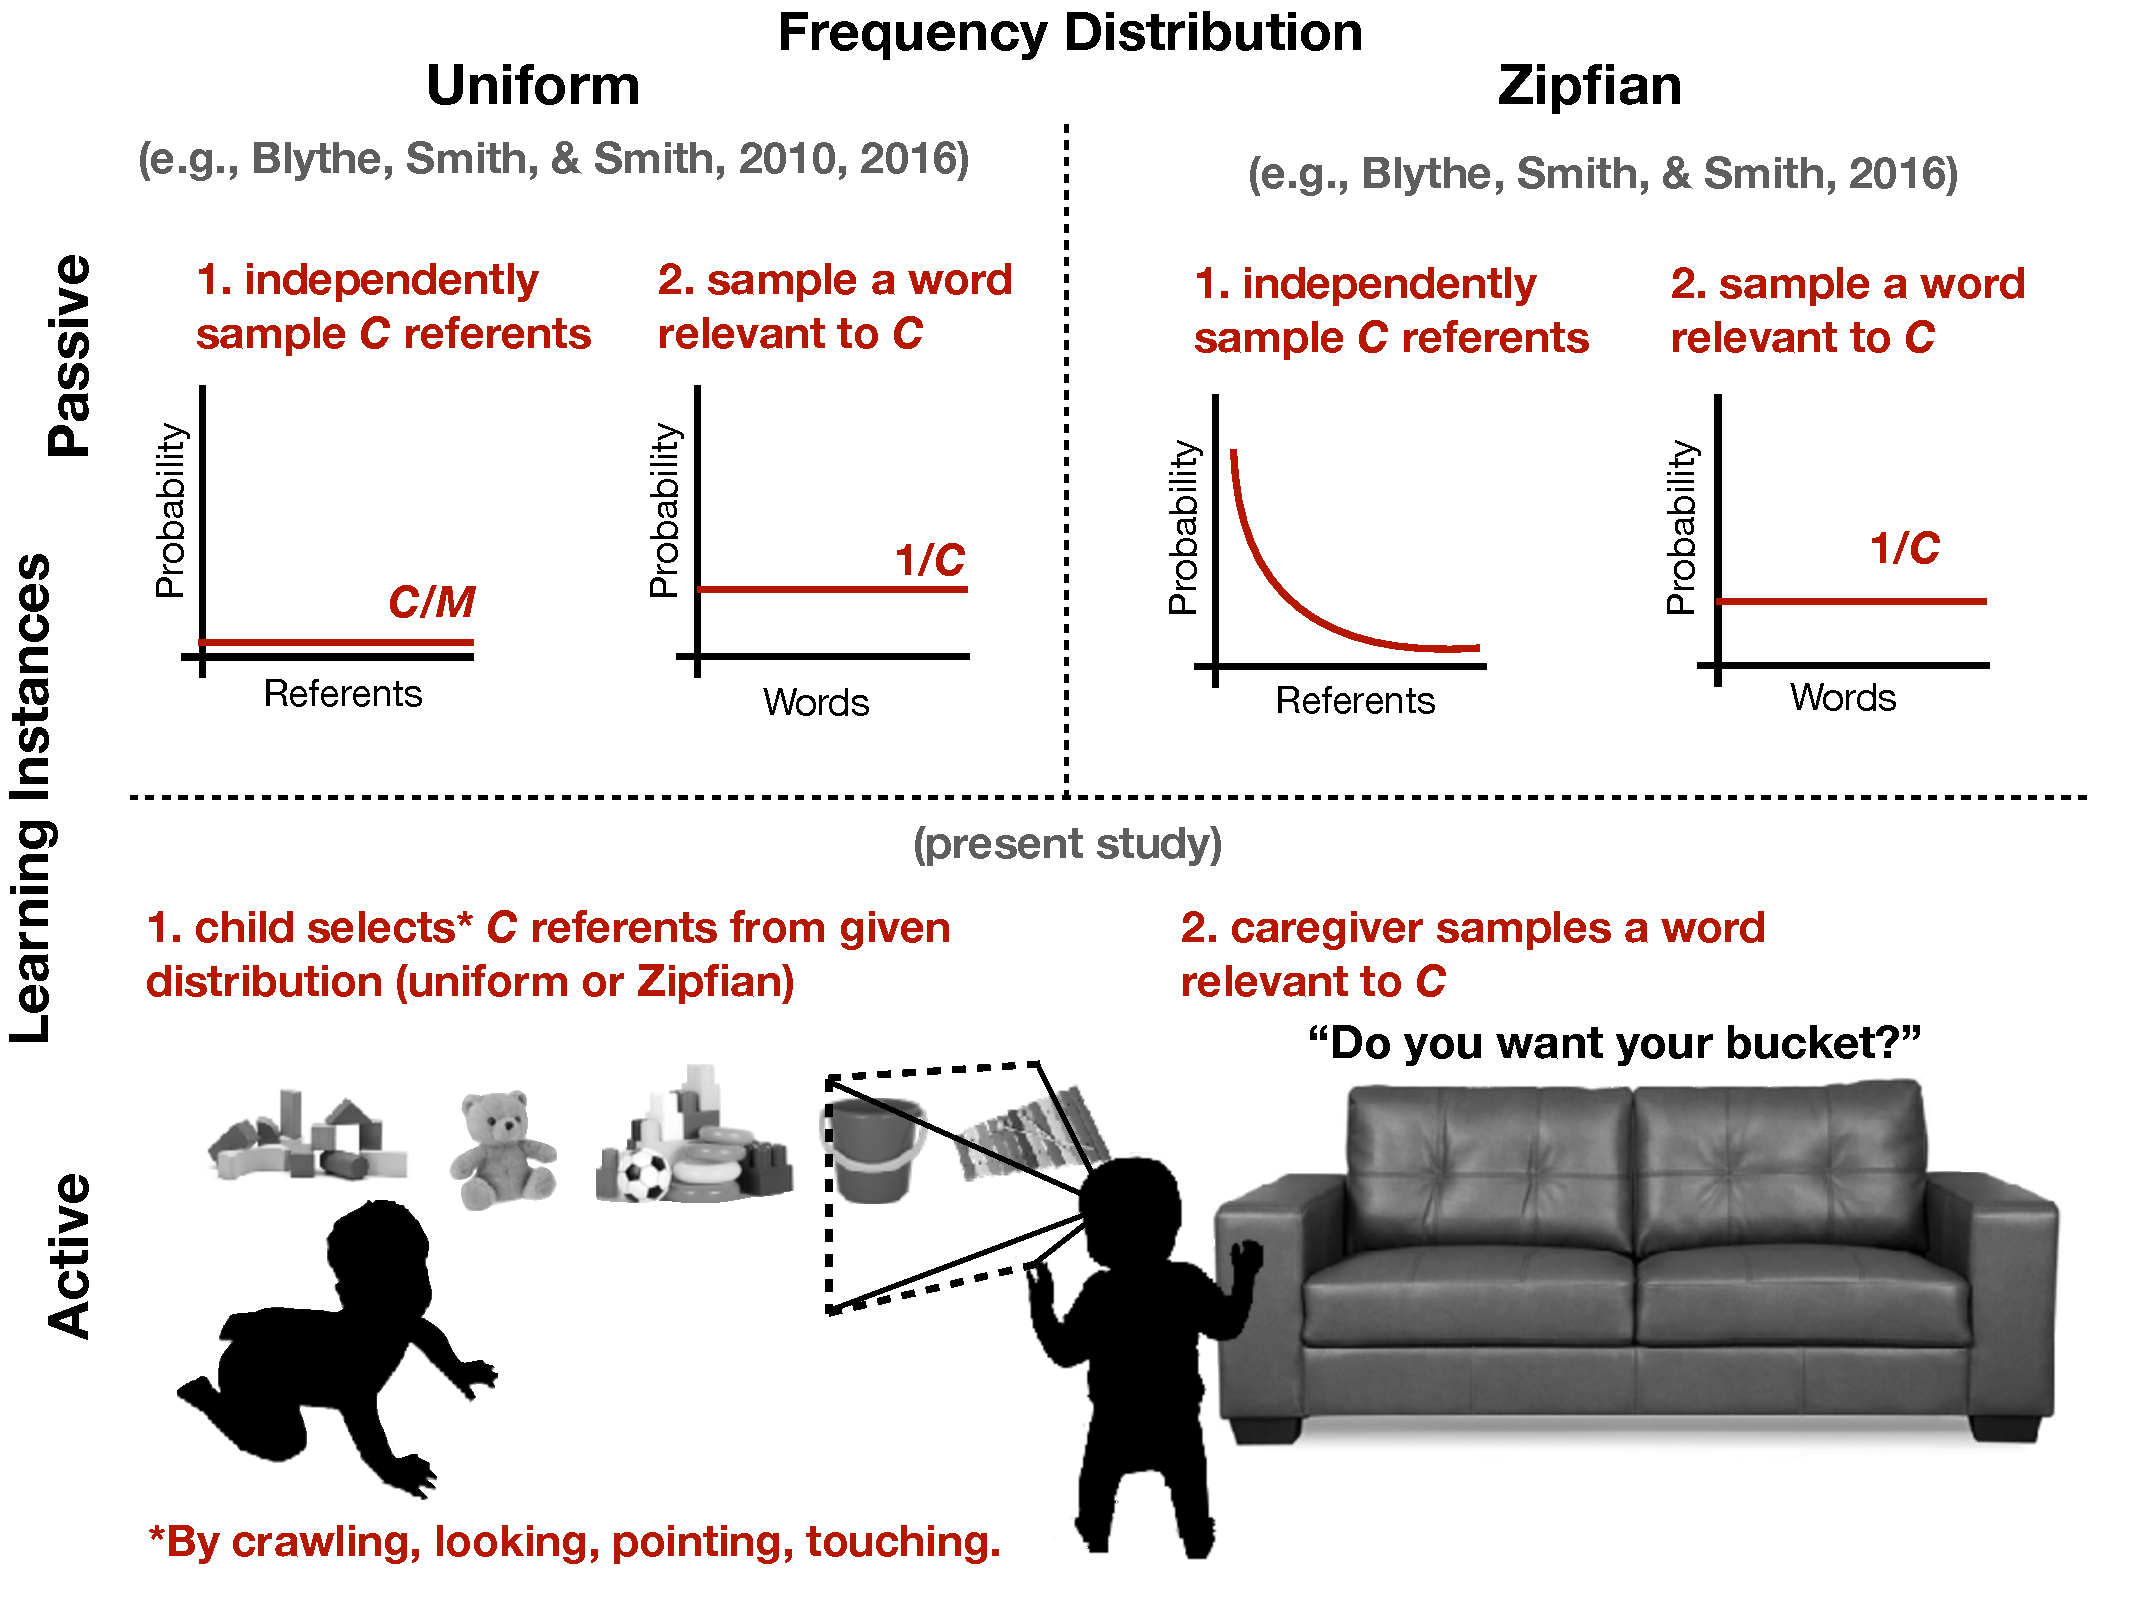
\includegraphics[width=\linewidth]{fig1-distros_vs_active_v2}
\caption{\label{fig-overview} 
  Previous research considered passive learning from independent random samples from uniform (top left) or Zipfian (top right) word and referent (i.e., meanings $M$) frequency distributions. The present work shows passive learning given a Zipfian word and referent distribution is too slow, and finds a solution in an analysis of a general form of active learning by which the infant (or caregiver) chooses the situation (i.e., context $C$) from which they will learn (bottom). }
\end{center}
\end{figure}

Given the difficulty of learning naturally-occurring Zipfian WFDs even with the power of fast-mapping, we explore an extension of the word learning mechanism by additionally assuming that early word learning is more {\it actively} directed by the learner than is typically assumed. 
In past analyses \citep[e.g.,][]{Blythe:2010,Vogt:2012,Blythe:2016}, the learner is passively observing randomly-selected words and referents from a given distribution. 
Motivated by diverse research on curiosity-driven learning \citep[cf.][]{Oudeyer:2016,Smith:2018}, we suggest that children are {\it active learners}, choosing to some extent what situation they would like to learn from at each moment (see Figure~\ref{fig-overview}).
Various forms of active learning have been studied in machine learning for online, incremental learning scenarios \citep[cf.][]{Settles:2012}, where it can generally outperform random sampling methods in classification tasks. 
Several behavioral studies of adults have found similar advantages for human active learners in tasks ranging from category learning \citep{Markant:2016} to word learning \citep{Kachergis:2013}, with children also showing benefits for active control \citep{Partridge:2015}.
% mention active learning in education (e.g., Montessori; Nolan, A., Kilderry, A., and O'Grady, R. (2006). Young children as active learners, Early Childhood Australia, Watson, A.C.T.)
Thus, we additionally analyze the impact of the learner actively structuring their word learning situations: choosing the referents from which a caregiver will select a target referent to name. 
Our analysis shows that this form of active learning enables sufficiently fast word learning for real-world timescales, even under a long-tailed Zipfian WFD. % and referent distribution

% Vogt:2012 - Fig. 4 shows that when C/M=0.1, the learning time t~=10^8, which in 18 years would amount to 15,221 words per day. When C/M 1⁄4 0.2, however, the learning time t~=2.9x10^9, which comes to about 441,400 words per day in 18 years. Assuming the upper bound of the number of words that parents are estimated to speak to their children (Hart & Risley, 2003), when hearing 2,100 words for 7.2 h per day, learning 60,000 words in 18 years is feasible with XSL, if C/M 1⁄4 0.1. However, children would require 210 h of input per day if C/M=0.2. Clearly, the former situation is plausible, and the latter is not.

\section{Methods}
abstract defining the ingredients

\section{Independent fast-mapping learning}

\subsection{Uniformly-distributed word frequency}
\cite{Blythe:2010} proposed a mathematical model of cross-situational word learning which has a closed-form expression under a certain simplification.
In their recent study, \cite{Blythe:2016} analyzed essentially the same model, slightly modified for analytic convenience.
Under this model, let there be $W$ words and $O$ referents in the hypothetical world, and let the number of words be equal to the number of referents, $W = O$. 
Furthermore, let the word-referent mappings be mutually-exclusive: each word corresponds to one (and only one) referent, so there are $W$ correct word-referent pairs.
Without loss of generality, denote the $W$ pairs by $1, 2, \ldots, W$, and suppose the $k^{\text{th}}$ referent is paired with the $k^{\text{th}}$ word.

Starting with these unknown words and referents, the learner is to infer correct pairs by experiencing {\it episodes}.
In each episode, the learner is exposed to one word $w_{k}$, and $1 < M < W$ referents, including the target referent $o_{k}$, but without any explicit information about the intended mapping of $w_{k}-o_{k}$. 
%\todo[inline, color=green!40]{different than Blythe et al, where M referents appear but only a single (random) referring word is selected. but just a smaller number of episodes by a factor of M.}
%If an episode presents $M \ge 2$ referents and words, the learner cannot tell which of $M$ words should be associated to which of $M$ objects.
%% (removed a paragraph about eliminative learning) 
%The learner, however, can infer the correct pairs of words and objects across multiple episodes, if a word is more likely to be spoken with the corresponding object present in the episode.
%In their analysis, they assume that the $k^{\text{th}}$ word is always spoken, if the $k^{\text{th}}$ object is present in the episode.
%Under this always-correct-word-spoken condition, the learner eliminates the possibility 
The simplest scheme is a fast-mapping learning model, which assumes one-shot learning: in one exposure the learner can map a new label to the correct referent. 
%, in which the learner is exposed to only one pair of object and word in each episode (or the learner can always infer there is a unique correct pair among other distractors).
%Empirical studies have found that children as young as three years old can quickly generalize a novel name to objects when they hear the novel name given to its first instance \citep{Spiegel:2011}. 
%A fast-mapping learner is equivalent to the cross-situational learner, if there is one correct pair of object and word in each episode ($M=1$).

As fast-mapping learning is the most efficient scheme for independent word learning, it gives a good baseline estimate of the number of samples to learn all the words in a vocabulary.
\cite{Blythe:2010} model a fast-mapping learner acquiring words independently drawn from a uniform distribution of $W$ words given in each episode.
As the probability of a given word in one episode is $1/W$, this is equivalent to the so-called Coupon Collector's Problem \citep{Blom1994}, which asks how many coupons one needs to draw with replacement before having drawn each of $n$ coupons (words) at least once. 
In this problem, the expected time $T$ to finish sampling all the words is 
%\[
% E[T] = \sum_{i=1}^{W} E[ t_{i} ].
%\]
%where $t_{i}$ is the time to sample a $i^{\text{th}}$ new word given $(i-1)$ words being learned.
%Thus, 
\begin{equation}
\label{eq-fastmap-T}
 E[T] = W \sum_{i=1}^{W} 1/i \approx W \log W. 
\end{equation}
For an adult-sized vocabulary $W = 60,000$, the estimated number of samples needed would be $T = 660,126$. % compared to Blythe:2010 estimate of 940,000 samples
This estimate is comparable with the ``reasonable'' number of samples justified by \citeA{Blythe:2010} which individual children can be exposed to for their 18 years of life.
% number of exposures suggested by Hart and Risley (2003): 2,100 words per hour, 14 h of exposure per day for 18 years (probably an upper bound as suggested by Blythe et al 2010; Mike Frank suggests 1,000 per hour, if I remember correctly)

\subsection{Number of samples for a general WFD}
We now extend this analysis of fast-mapping to the more realistic case of non-uniform WFDs.
This analysis will reveal that the estimate based on Equation (\ref{eq-fastmap-T}) by Blythe et al. is overly-optimistic: learning of non-uniform distributions is generally much slower.

%\todo[inline, color=green!40]{Details of the following few paragraphs are moved to Appendix 1.}
Suppose a set of $W$ words in which each word $1, \ldots, W$ is drawn from the distribution $p = (p_{1}, \ldots, p_{W})$.
Let us write the number of episodes by $T$ which is required to have
the proportion of children who finished learning all the words is $(1 - \epsilon)$ for $0 \le \epsilon \le 1$.
For the uniform distribution, $p_{i} = 1/W$ for every $i = 1, \ldots, W$, the number of samples is 
\begin{equation}
\label{eq-T}
 T = f_{W, \epsilon}( 1/W ),
\end{equation}
where
\[
 f_{W, \epsilon}( x ) := 
\frac{ 
  \log\left( 1 - ( 1 - \epsilon )^{1/W} \right) 
}{ 
  \log\left( 1 - x \right) 
}.
\]
Setting $\epsilon = 1/2$ in (\ref{eq-T}), we obtain the median of $T$, $f_{W,1/2}(1/W)$, that is comparable with the mean of $T$ in (\ref{eq-fastmap-T}).

Unlike (\ref{eq-T}) for the uniform distribution, the number of samples $T$ for an arbitrary WFD in general does not have a closed-form solution.
Thus, instead of the exact expression of $T$, we consider the upper and lower bound for $T$ (see Appendix 1 for the derivation).
For the general WFD $p = (p_{1}, \ldots, p_{W})$, we have inequality

\begin{equation}
f_{W, \epsilon}( \max p ) \le T \le f_{W, \epsilon}( \min p ) := T_{+}.
\label{eq-Tbound}
\end{equation}

As we are interested in the worst possible estimate of $T$, this inequality states that 
the upper bound $T_{+}$ of $T$ is characterized with 
the probability to sample the least frequent word $\min p$.

\subsection{Impact of non-uniform word frequency}
This extended mathematical analysis implies that the uniform distribution $q = (1/W, \ldots, 1/W)$ of words gives the minimal possible upper bound $T_{+}$ among any WFD of $W$ words, 
as any distribution $\min p$ of $W$ words holds $\min p \le \min q$.
Therefore, the expectation of $T$ in the form of (\ref{eq-fastmap-T}) with uniformly-distributed words is the most optimistic, and thus likely underestimates the number of episodes required for learning a realistic WFD.

For example, consider the case that the $W$ words are Zipf-distributed with exponent $a \ge 0$ defined by 
$$p = (1^{-a}/H_{W,a}, 2^{-a}/H_{W,a}, \ldots, W^{-a}/ H_{W,a})$$
where $H_{W,a}$ is the generalized harmonic number $H_{W,a} = \sum_{i=1}^{W}i^{-a}$.
%the Zipf distribution $$p = (1^{-1}/H_{W}, 2^{-1}/H_{W}, \ldots, W^{-1}/ H_{W}),$$ where $H_{W}$ is the harmonic number $H_{W} = \sum_{i=1}^{W}i^{-1}$.
With $a = 0$, this reduces to a uniform distribution.
The larger the exponent $a$ is, the minimal probability $\min p$ is smaller.
In the case of the ``standard'' Zipfian distribution $a=1$, the minimal probability is $\min p \approx 1.44 \times 10^{-6}$,
and the upper bound $T_{+}$ is $1.08 \times 10^{7}$ for $\epsilon = 0.01$.
This estimate means that learning a Zipfian WFD requires 16.4 times as many samples as learning a uniform WFD. % compared to Blythe 2010s: 11.58x slower for 60,000 words
This implies 206 independent episodes exposed to a word learner per hour--three episodes every minute--assuming 8 hours of learning everyday of 18 years of life. % 206*8 * 365 * 18 = 10,827,360 episodes; 
This number of independent episodes does not seem reasonable with respect to the ordinary life of children in any culture. % Piantadosi estimates of Effective Learning Instances?


%\todo[inline, color=green!40]{Details of the Section ``Sensitivity to non-uniformity of word frequency distribution'' are moved to Appendix (2?)}
\subsection{Sensitivity to non-uniformity of word frequency distribution}

To analyze how sensitive the number of samples $T$ is to non-uniformity, we analyze Zipfian WFDs with different exponents.
%Denote the Zipf distribution with the exponent parameter $a \ge 0$ 
%by $p = (1^{-a}/H_{W,a}, 2^{-a}/H_{W,a}, \ldots, W^{-a}/ H_{W,a})$
%where $H_{W,a}$ is the generalized harmonic number $H_{W,a} = \sum_{i=1}^{W}i^{-a}$.
With some calculation (see Appendix 2), we find the upper bound $T_{+}$ (Equation \ref{eq-Tbound}) as a function of the exponent parameter $a$ holds the bound
\[
 \frac{\partial^2 \log T_{+} %f_{N, \epsilon}( p_{\min} )
 }{ \partial a^2 }
\ge 0.
\]
This implies the $T_{+}$ is a super-exponential monotone function of the exponent $a$. % can this be compared to Vogt:2012 findings?
It is also numerically confirmed in Figure~\ref{fig-estimate}, which shows the number of episodes as a function of the WFD's exponent for $W = 10000, 60000$.
In this plot, $a=0$ shows an estimate for the uniform distribution, and $a=1$ shows that of the standard Zipfian distribution.
It is striking that even fast-mapping--the most efficient learning--can be quite slow (exponentially as a function of $a$) for distributions that have some low-probability items.


\begin{figure}[h]
\begin{center}
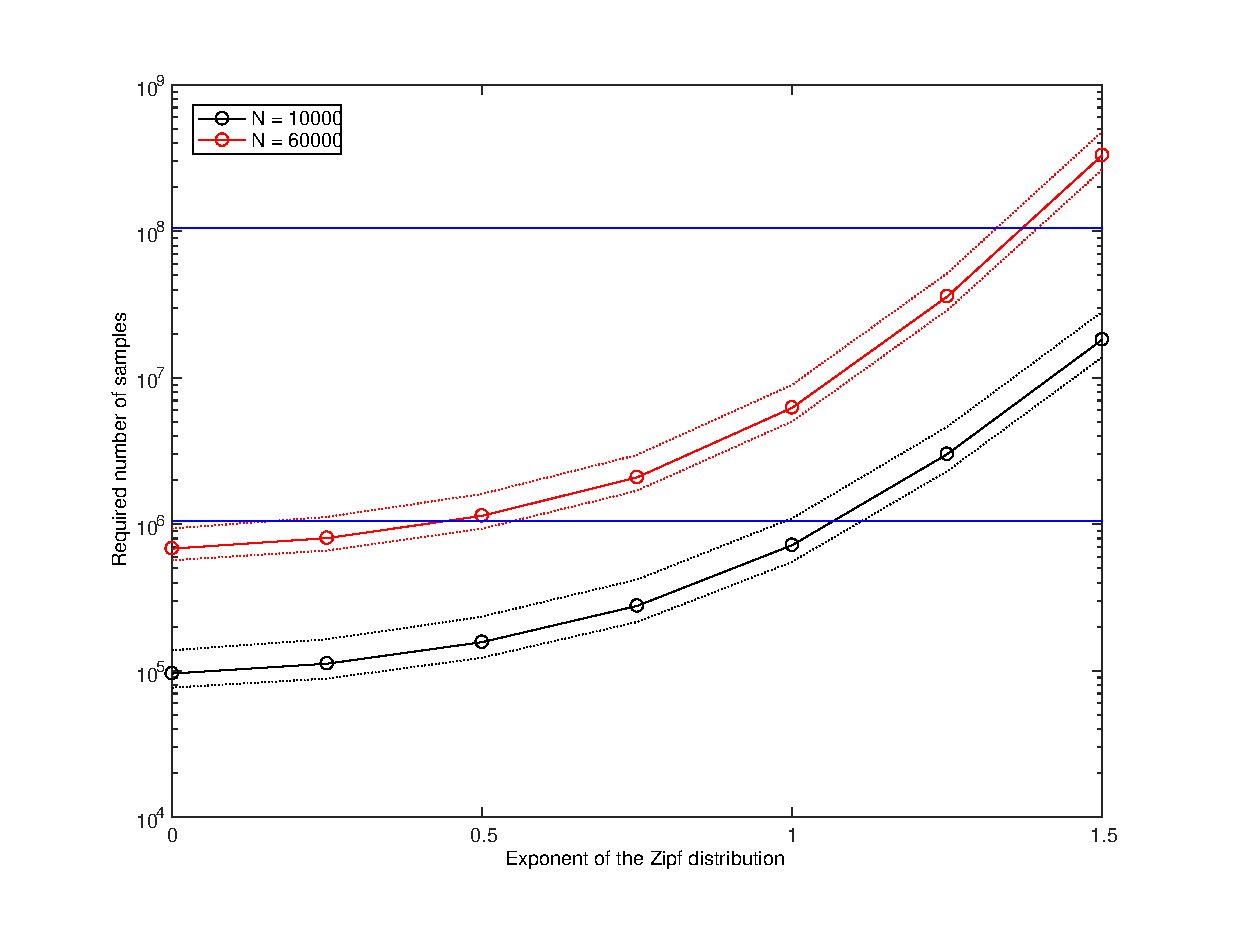
\includegraphics[width=\linewidth]{Summary2.eps}
\caption{\label{fig-estimate} 
The required number of samples ($M$) from a generalized Zipf distribution ($p_{k} = k^{-a}/\sum_{k=1}^{N}k^{-a}$) needed for 1\%, 50\%, and 99\% of learners ($\epsilon$ = [.99, .01]; dotted lines, $\epsilon$ = 0.5; solid line) to reach a vocabulary size of $N = 10000$ or $N = 60000$, for varying values of the distribution exponent $a = 0, \ldots, 1.5$. A value of $a = 0$ corresponds to a uniform distribution. The number of samples is numerically calculated by the root of Equation (\ref{eqA-M}) in Appendix 1.} % what's the empirical a for CHILDES? ~1.5?
\label{fig}
\end{center}
\end{figure}
% (\ref{eqA-M})

\subsection{Empirical dataset} % Shohei, maybe we should just refer to your other paper's estimate of the CHILDES exponent?
Given these theoretical implications, we analyze an empirical WF distribution of child-directed speech in the CHILDES corpus \citep{MacWhinney1990}.
%It is difficult to exactly count ``episodes'' or ``pairs of word and object'' in a real dataset, due to its ambiguity of definition and it is also up to children's subjective perspective.
%Here, as a proxy of them, we counted the word frequency based on child-directed speech in the CHILDES corpus \cite{MacWhinney1990}. 
Figure~\ref{fig-freq} shows a representative word distribution of 51,446 words aggregated over 4,163 transcripts from CHILDES (retrieved December 2007).
The minimal word probability was $1.089 \times 10^{-7}$, which gives the upper bound $T_{+} = f_{51446, 0.01}(1.089 \times 10^{-7}) = 1.420 \times 10^{8}$
or the median estimate $T_{+} = f_{51446, 0.5}(1.089 \times 10^{-7}) = 1.030 \times 10^{8}$. These estimates of required samples, being an order of magnitude larger than the optimistic theoretical estimate, suggest that this empirical Zipfian WF distribution would be difficult to learn.
%% See also test_fastmap.m in the XSL folder for more detail.

\begin{figure}[h]
\begin{center}
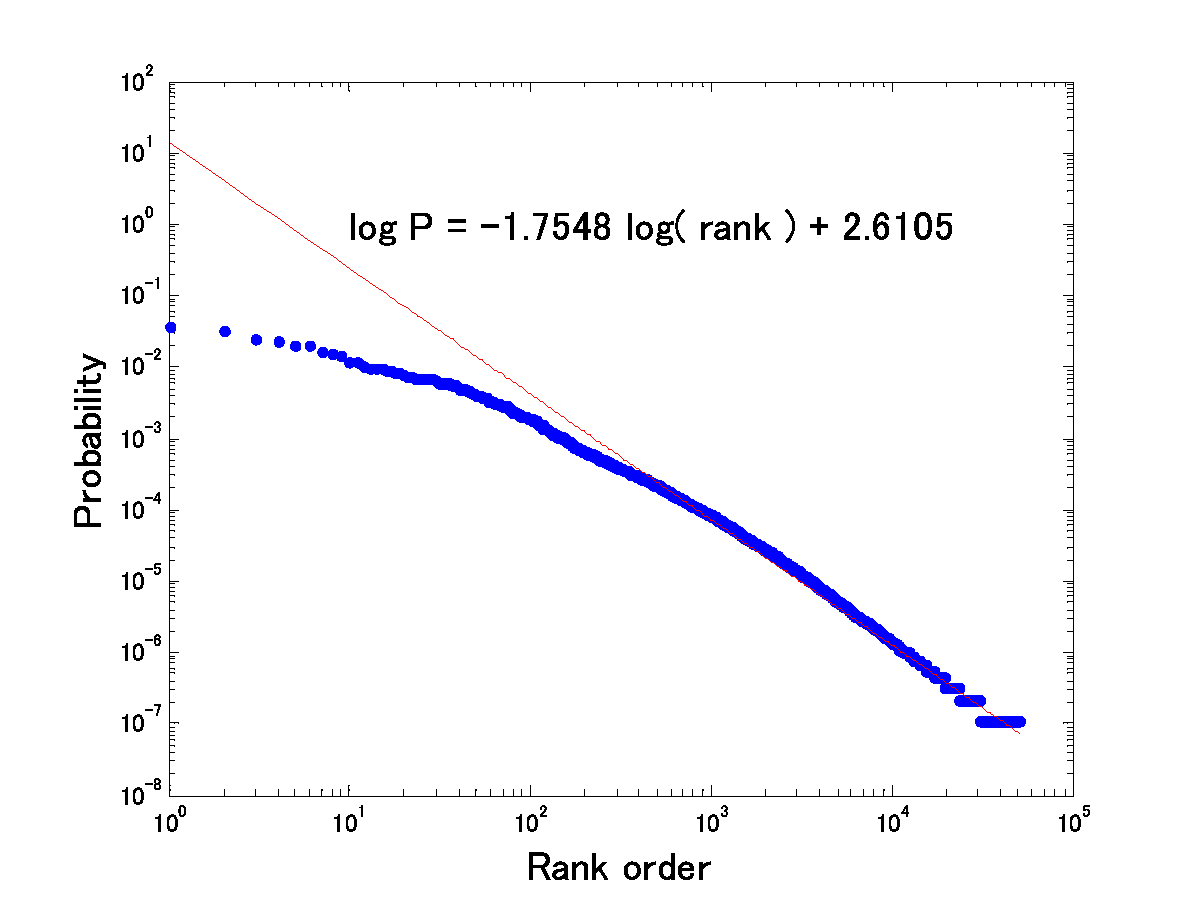
\includegraphics[width=\linewidth]{FreqCHILDES.eps} % width=9cm
\caption{Word frequency in the CHILDES corpus transcripts.}
\label{fig-freq}
\end{center}
\end{figure}

%% Shohei added this section on Nov 9th, 2016.
\section{Active learning: Choosing situations}
\subsection{Formulation}
The mathematical analysis above suggests that even the power of fast-mapping may not be efficient enough to learn Zipfian WFDs, raising the question of what mechanisms enable children to learn the nonuniform distributions they experience.
We explore one way to reconcile this discrepancy by adjusting the assumption about how about meanings are sampled in each situation.
In the analysis so far, the learner is assumed to be {\it passive}, having no choice but to observe and learn from a given situation: a randomly-sampled set of of objects, of which a (random) subset are labeled with words. 
The simplifying assumption of a passive learner likely underestimates real learners (and caregivers), who have some control over which situations are experienced.
Here, we consider a type of active learner who is able to {\it actively} choose the situations from which she learns words. 

Suppose that there are $N$ word-referent pairs and $M$ situations, and that the conditional probability to observe the $i^{\text{th}}$ word-referent pair is $p_{ij}$ given the $j^{\text{th}}$ situation. 
Assume the active learner can choose the next learning situation from the given $M$ situations. %from which she learns the word-referent pairs. 
Suppose that the active learner chooses the $j^{\text{th}}$ situation with probability $q_{j}$.
Denote the $N \times M$ matrix of conditional probabilities by $P = \{ p_{ij} \}_{ij}$ and the $N \times 1$ vector of the situation choice probabilities by $q = (q_{1}, q_{2}, \ldots, q_{M})^{T}$.
Thus, the marginal probability of word-referent pairs is given by the vector $Pq \in \mathbb{R}^{N}$.
According to the analysis in the previous section, the minimal probability of referents (or words) determines the number of samples required to complete the word learning, meaning
the best choice for the active learner is given by the choice probability \footnote{In the context of game theory, this optimal $\hat{q}$ corresponds to the max-min strategy (or Nash equilibrium) for the two-player zero-sum game defined by the payoff matrix $P$ (see for instance \cite{Maschler:2013}). } 
\[
 \hat{q} = {\arg\max}_{q} \min(Pq).
\]
This minimal probability, $\min(P\hat{q})$, gives the theoretical upper bound for the minimal number of samples $$T_{+}=f_{W,\epsilon}( \min(P \hat{q}) ).$$
This is an upper bound with the known $P$, because the probability matrix
$P$ is not known before empirical learning, and the active leaner also needs to estimate $P$ from the sample.

For a given matrix $P$, the optimal $\hat{q}$ can be computed by the iterated linear programming algorithm (see Appendix 3 for details). % algorithmic complexity of this? Iris van Rooij and Johan Kwisthout would care

As a baseline for the passive learner, we consider the average $\min( Pq )$ with the uniform distribution over the vector $q$, whose lower bound is given by Jensen's inequality $$\int_{q\in \Simplex{N}}\min( Pq ) (N-1)!\dd q \ge \min( P \one{N}/N ),$$
where the integral is taken over the $N-1$ dimensional unit simplex $q\in \Simplex{N}$.
For a sufficiently small $x \ll 1$ and $y \ll 1$, $f_{W,\epsilon}(x)/ f_{W,\epsilon}(y) \approx y/ x$.
Thus, the rate $$R = \min(P \hat{q})/ \min(P \one{N}/N)$$ gives a good estimate for the rate of efficiency, by which
active learning with the optimal probability $\hat{q}$ is $R$ times faster on average 
than passive learning with a uniformly-randomly chosen probability vector $q$. % transition sentence explaining what we do

\subsection{Empirical evaluation}
% from Takuma's presentation: 131067 Images, 908 Scene categories, 313884 Segmented objects, 4479 Object categories
To evaluate the potential impact of active leaning, we study the SUN database \cite{SUN2010} as an empirical estimate of object distributions in a collection of real-life scenes. 
The SUN database (retrieved September 25, 2016) has $N = 3,458$ objects and $M = 1,111$ representative indoor and outdoor scenes in 131,067 images. 
This data gives an estimate of the $N \times M$ matrix $P$ in which each column is the conditional probability of the objects given each scene. 
With uniform scene choice probability $q = \one{N}/N$, the $\min(Pq)$ is $8.30\times 10^{-9}$. 
Meanwhile, with the optimal $\hat{q}$, the $\min(P\hat{q})$ is $1.95\times 10^{-6}$, indicating active learning is approximately $R = 235.3$ times faster than the baseline passive learning. 
The marginal probability distributions of objects for the baseline and optimal $q$ are shown in Figure \ref{fig-optimalQ}. 
The difference between the two marginal distributions is visible at their tails: the tail of the uniform $q$ decreases like an exponential function, but that of the optimal $\hat{q}$ decreases as a power function (linear in the log-log plot).
This empirical evaluation suggests that this form of active learning can make fast-mapping orders of magnitude more efficient.

\begin{figure}[h]
\begin{center}
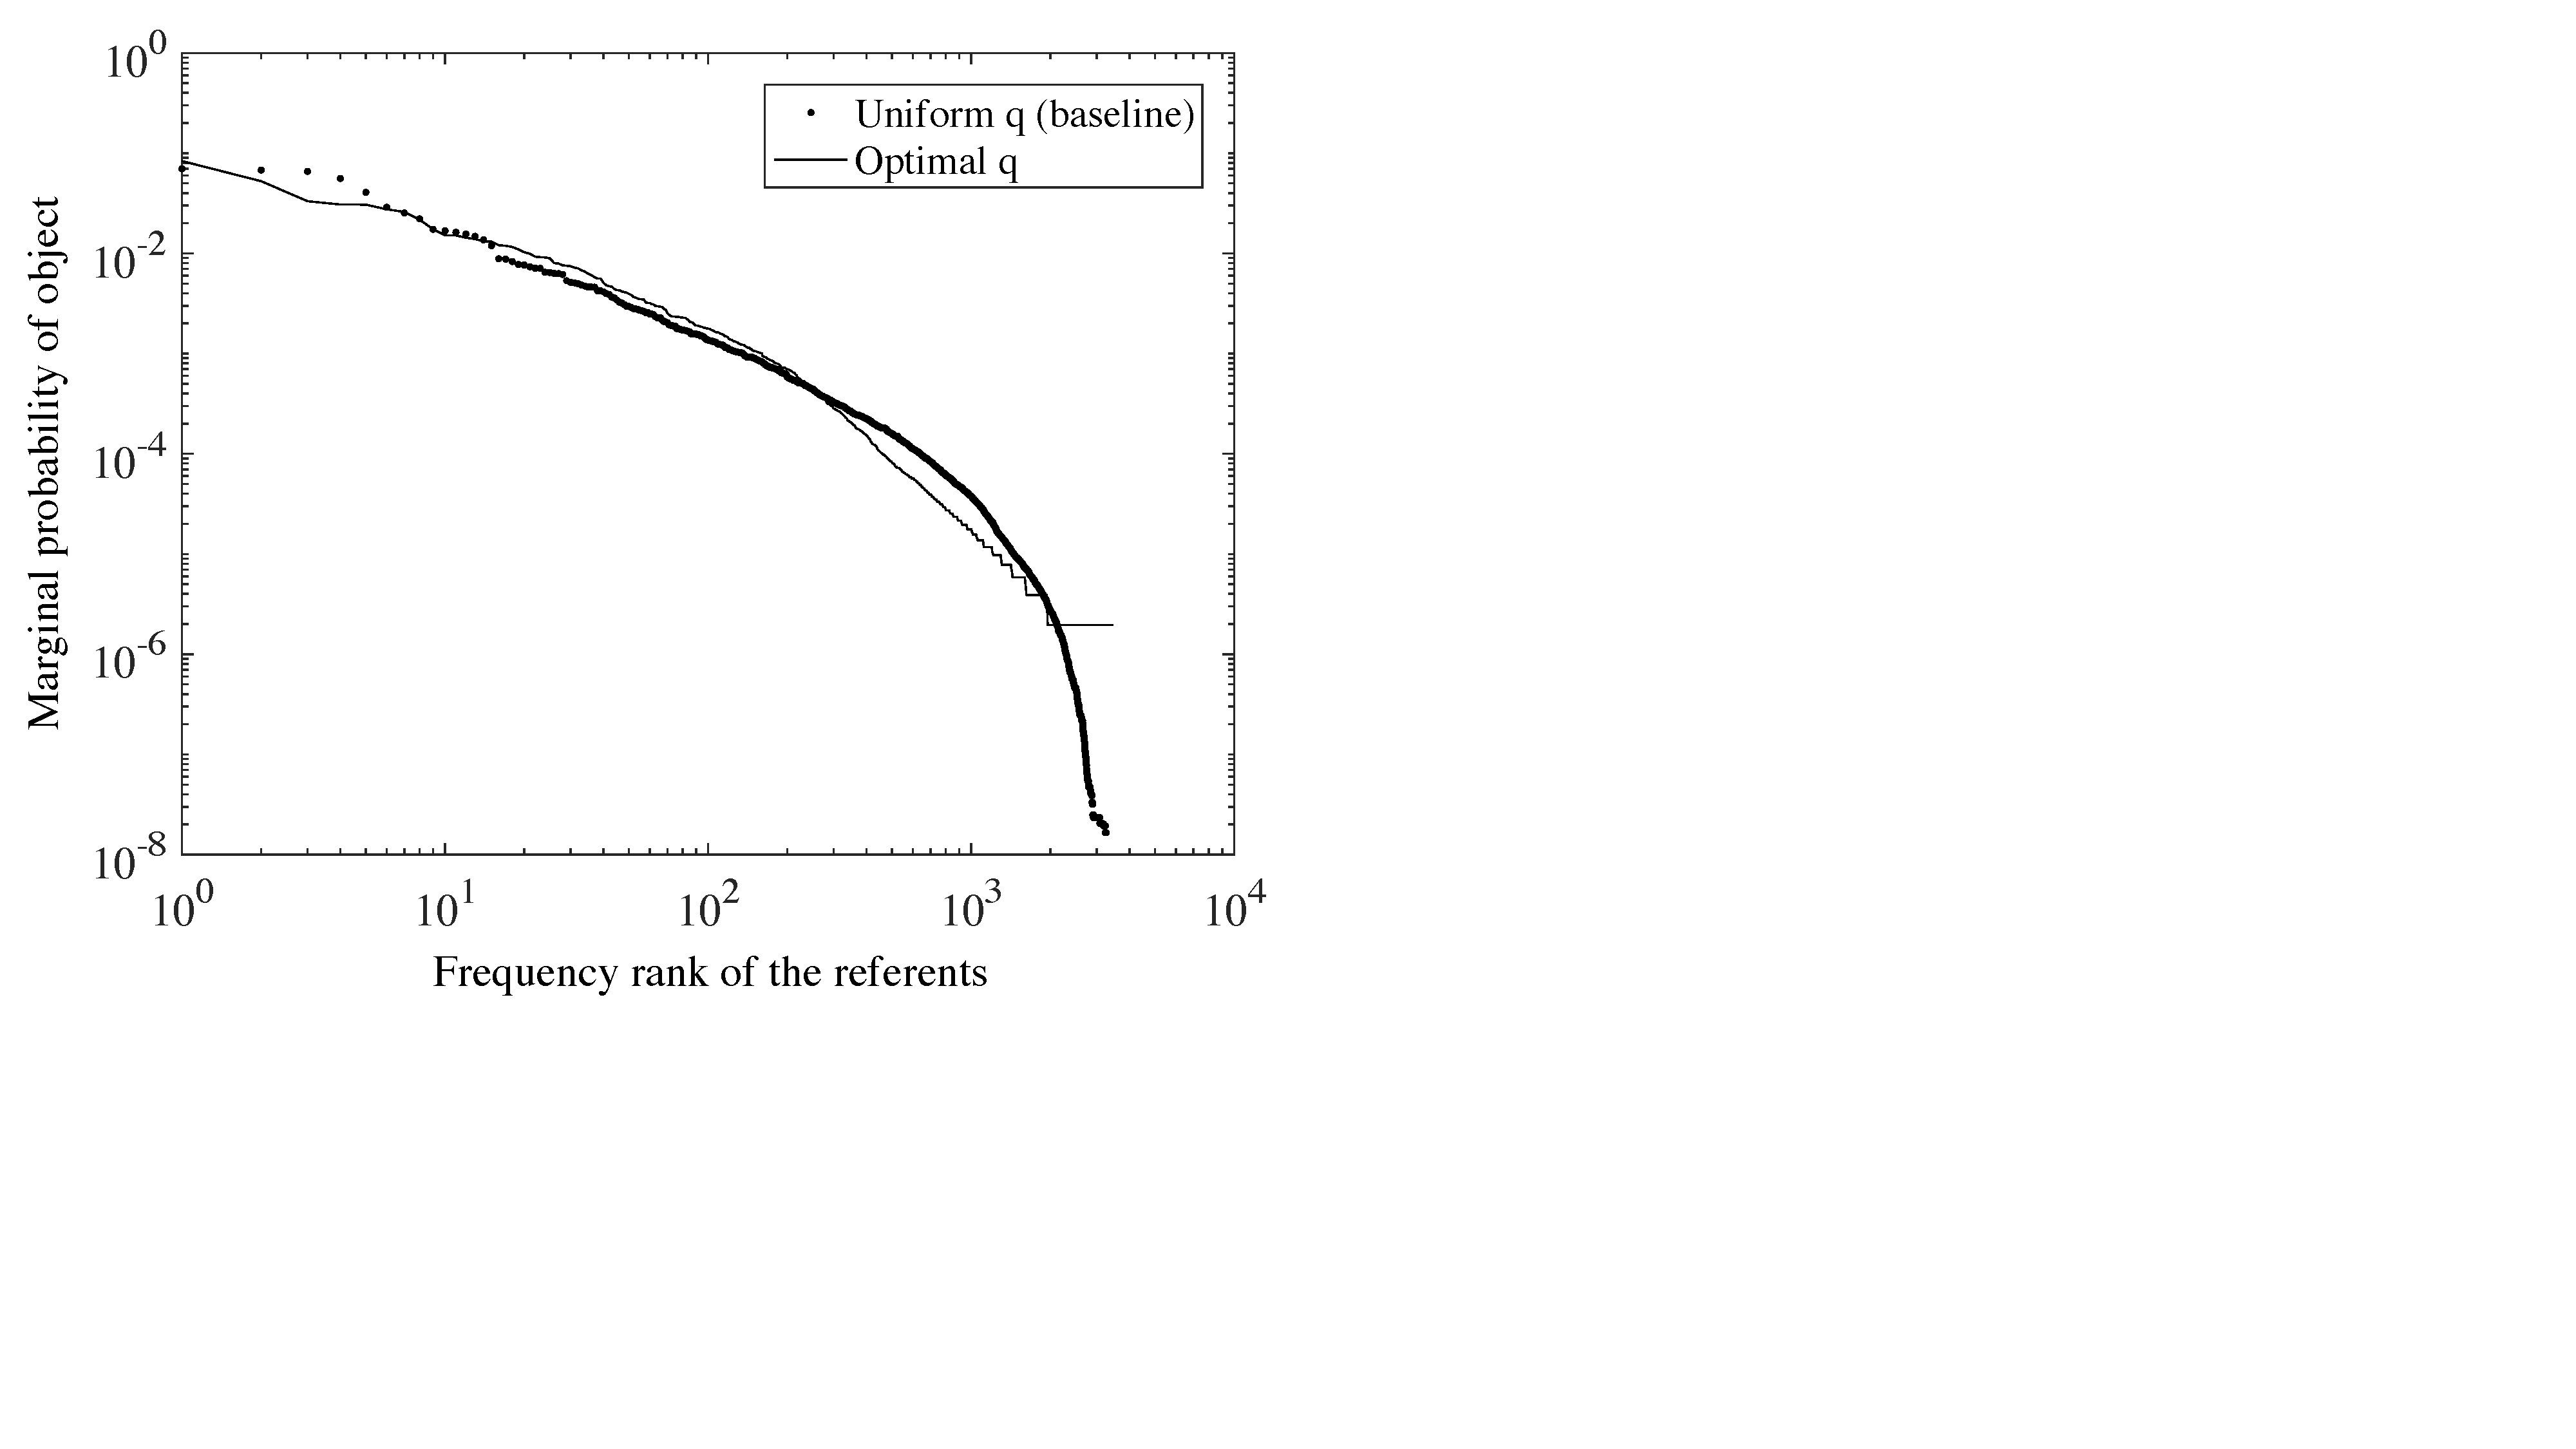
\includegraphics[width=\linewidth]{OptimalQDistribution3.pdf}
\caption{The marginal probability of referents for the optimal $\hat{q}$ (line) and its baseline (dots).}
\label{fig-optimalQ}
\end{center}
\end{figure}

\subsection{Online active learning with an unknown $P$}
%\todo[inline, color=green!40]{As Reviewer 3 misunderstand this and previous section, Shohei would clarify these sections.}
The above measure of active learning's efficiency is based on the optimal $\hat{q}$ with full knowledge of $P$, which gives an optimistic estimate of learning time since the matrix $P$ is unlikely to be fully known to the learner. 
Thus, we perform a Monte Carlo simulation to quantify the efficiency of an {\it online} active leaner who gradually learns $P$ and estimates $q$ based on the sample estimate of $P$. 
If this online active leaner is comparable to the optimal active learner with $\hat{q}$, we can treat the performance analysis of the optimal active leaner above (a few orders more efficient) as holding for the online active leaner. 
For this purpose, we generated a $N \times M$ matrix $P$ with $N=1000, M=100$, which has the elements in each column are Zipfian probabilities $P_{\pi(i)} \propto i^{-a}$ with random coefficients $a \in [1, 1.5]$, where $\pi: \{1, \ldots, N\} \mapsto \{1, \ldots, N\}$ is a random permutation. 
The online active learner has uniform choice probability $q_{1} = \one{N}/N$. 
For $k^{\text{th}}$ batch of 1000 steps, the online learner samples the objects according to the probability $P q_{k}$, and constructs the sample probability matrix $\hat{P}_{k}$ according to sample frequency. 
After the $k^{\text{th}}$ sampling step, the online learner estimates $q_{k} := \argmax_{q} \min( \hat{P}_{k} q )$. 
In each run of this procedure, we repeat up to $100 \times 1000$ samples, and obtain one sample for the number of required samples to finish learning names for all of the 1000 referents--the approximate vocabulary size of a 3-year-old. 

With 100 runs, we obtain the Monte Carlo estimate of the online learner shown in Figure \ref{fig-online}.
Figure~\ref{fig-online} shows the sample probability distribution of the number of required samples in the Monte Carlo simulation (circles: histogram, line: smoothed estimate), and its comparable median estimate for the optimal learner (green vertical line) and the passive learner with the uniform $q$ (red vertical line).
This simulation result shows that the online learner is, on average, as fast as an optimal learner, and is almost always faster than the passive learner, which requires twice as many samples.

Beyond the case study reported above, we also provide a theoretical analysis of why such online learning is possible in Appendix 4.

\begin{figure}[h]
\begin{center}
%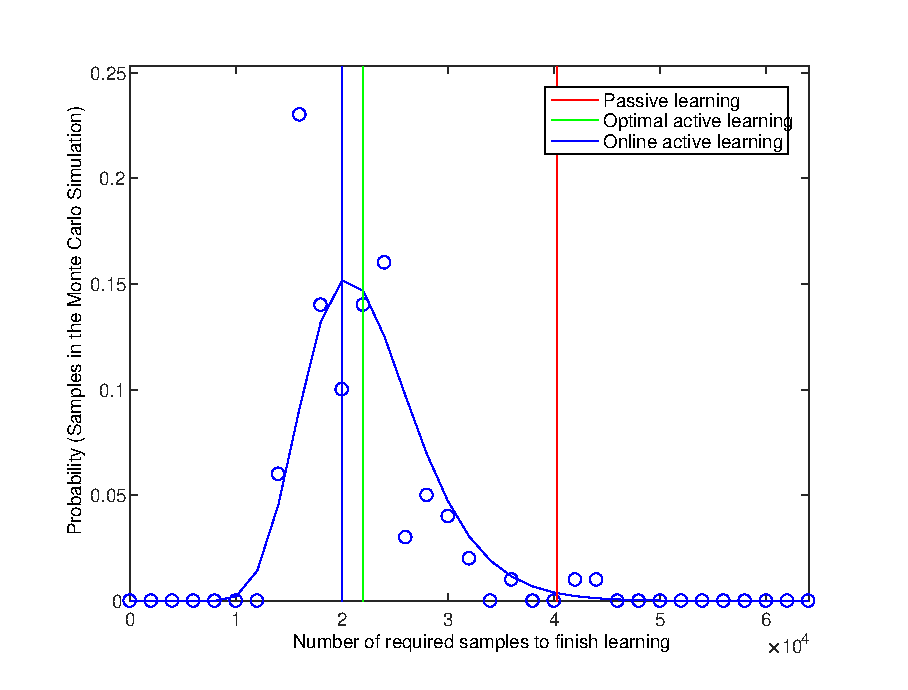
\includegraphics[width=9cm]{OnlineActiveLearning.eps}
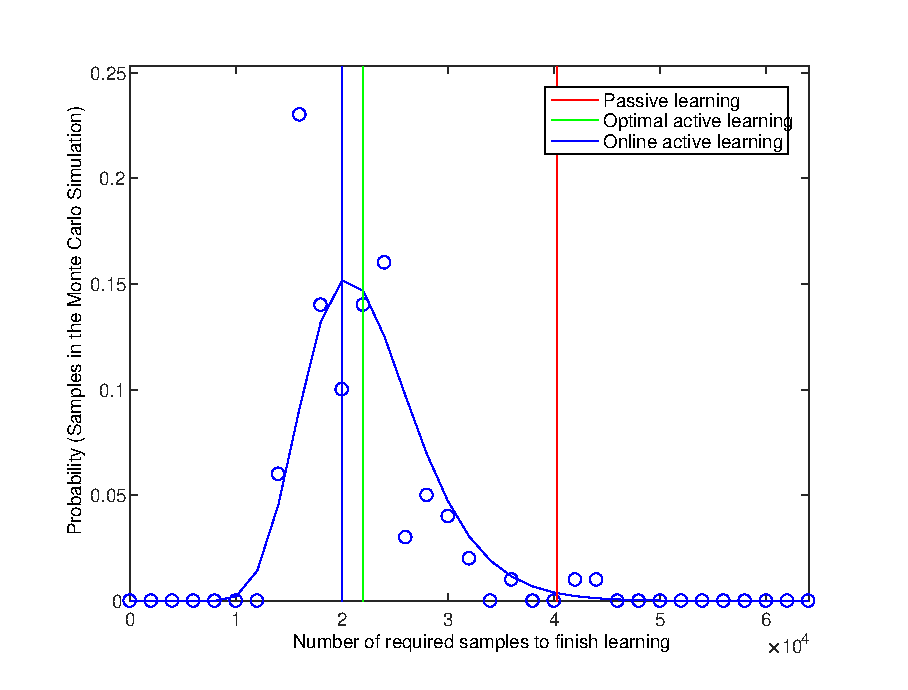
\includegraphics[width=\linewidth]{OnlineActiveLearning.eps}
\caption{The probability distribution of the number of required samples to finish learning for passive (red), optimal (green), and online active learners (blue). On average, online active learning was as fast as optimal active learning.}
\label{fig-online}
\end{center}
\end{figure}

\section{Discussion}

%This study offered a mathematical analysis of word learning, providing general constraints that any theoretical account of children's word learning should satisfy. 
This study reinspected the claim by \cite{Blythe:2010} that independently fast-mapping word meanings is efficient enough to learn a full adult lexicon in 18 years, under more realistic assumptions of Zipfian (i.e. power-law) word and referent frequency distributions, previously considered by \cite{Vogt:2012}. 
We offer a first analytical estimate for the learning time of an entire lexicon assuming nonuniform distributions of meanings and words, verifying \cite{Vogt:2012}'s conjecture that learning time for Zipf-distributed words and meanings depends on the number of meanings and the probability to sample the least frequent word or referent. % Vogt also suggested C - context size; incidental meanings - matters
Our new analysis showed that even learning via fast-mapping is not efficient enough to learn words whose distribution has rarely sampled words--including the Zipf distribution. % In essence, learners end up waiting a long time for the long tail of the distribution: low-frequency words are simply too rare.

% discuss relation to Hidaka2013 and MollicaPiantadosi2017 effective learning instances -- we define how ELIs might be constructed (for one-shot learners), while they estimate how -- constant factor (still reasonable amount of input?)
Given that our analysis implied learning would be too slow under realistic distributions, we considered a more efficient learning scheme, in which the learner can choose preferred learning situations by composing the contexts from which words are drawn. 
This type of active control over situations seems natural with respect to general observations of children's behavior \citep{Yu:2009active}, and has been shown to benefit adult word learners \citep{Kachergis:2013}, but has not to our knowledge previously been subjected to theoretical analysis. 
We quantify and evaluate the effect of this type of self-directed learning in word learning using a modeling framework with few assumptions \citep{Blythe:2010,Vogt:2012,Blythe:2016}. 
As the least probable word in the distribution determines learning efficiency, we analyzed the effect of active choice on the situations maximizing this key parameter. 
Analyzing an empirical dataset of labeled referents in a set of natural scenes, we found that the expected learning time of an active learner is over two hundred times more efficient than a passive learner. 
This result suggests that active choice in word learning is one possible resolution to the issue that passive learners cannot learn sufficiently quickly from naturalistic Zipfian distributions.
% We propose and analyze the learning time for a general active learning algorithm--including an online version. 

This paper analyzed fast-mapping--a simple yet powerful learning scheme--in order to highlight the effects of nonuniform word frequency distributions, with and without active learning. 
\GK{We expect that other word learning mechanisms suffer to the same extent from nonuniform distributions in the environment, and future work can use the same analytic techniques presented here to confirm that.
Moreover, we expect that the active learning mechanisms presented are generalizable to other models, and will similarly alleviate the difficulty of learning from naturalistic nonuniform distributions.
Although the optimal active learning algorithm we have considered may not be cognitively plausible (and thus may predict faster learning than young children show), in conjunction with the fast-mapping mechanism it offers an upper-bound on the speed of active word learning, and future work should consider suboptimal active learning mechanisms that are more cognitively plausible.}
Note that the general scene-selection algorithm analyzed here could be implemented by the child, the caregiver, or both as they jointly choose (or reject) referents and locales. 
\GK{Indeed, observations of parent-child free-play sessions have found that both parents and children often construct scenes with a single object dominating the child's visual field \citep{Yu:2009active}, with manual manipulations of both the parent and the child contributing to the visual clarity of the objects \citep{Suanda:2018}. 
Data such as these could be used to test the efficacy of various active learning mechanisms against real-world data, providing additional insights into how restructuring a child's environment might improve word learning.
Applying mechanisms of active learning to the rich and changing input will allow us to test the idea that infants create a curriculum for statistical learning \citep{Smith:2018}.
}

%As we analyze models with more realistic assumptions about the language environment, we also look forward to better empirical estimates of young children's ability to structure their learning environment.
%On this path towards ever more realistic assumptions about the language environment and learners' ability to shape it, we expect to make progress toward a general theoretical framework spanning many proposed word learning schemes.

%\todo[inline, color=green!40]{Relate to Effective Learning Instances? ELIs not yet defined, though}

% use section* for acknowledgement
\section*{Acknowledgment}
%This study is supported by the JSPS KAKENHI Grant-in-Aid for Young Scientists JP 16H05860.

\bibliographystyle{apacite}
\setlength{\bibleftmargin}{.125in}
\setlength{\bibindent}{-\bibleftmargin}
\bibliography{corpusXSL_refs}

\pagebreak



% \section{Appendix 0: Rate of word learning}
% % we don't currently refer to this Appendix: where should we?
% Suppose that $(1-p_{T})$ is the probability that the learner has learned all the $N$ words by observing $T$ samples of them. If there exists a quantity in the limit $$R := - \lim_{T \to \infty} \frac{\log p_{T}}{T},$$ we call it the rate of word learning. This definition of the word learning rate is motivated by information theory, in which the rate characterizes the exponential increase of the number of codes per letter for the triplet of the encoder, decoder, and channel.  Any word learning scheme with the rate $R$ implies that the learning error decreases exponentially, $e^{-RT}$, as the function of the number of samples $T$ in a long run. Thus, from the information-theoretic perspective, the class of word learning schemes with the same rate is {\it equivalent} with respect to the learning rate in a long run.

% With this rate $R$ of word learning, we identify any learning expressed in the form
% $$
% p_{T} = \lambda e^{ -RT + \Delta_{T} },
% $$
% where 
% where $lambda$ is a certain constant and $\Delta_{T}$ is a residual term holding $\lim_{T \to \infty }\frac{ \Delta_{T} }{ T } = 0$.

% Extending this idea, the error probability of fast-mapping learning is expressed in the form
% $$
% p_{T} = \lambda_{1} e^{-R_{1}T - \lambda_{2} e^{-R_2 T + \Delta_{T}} },
% $$
% where $\lambda_1$ and $\lambda_{2}$ are some constants, and $\Delta_{T}$ is a residual term holding $\lim_{T \to \infty }\frac{ \Delta_{T} }{ T } = 0$.
% With this definition, we have the following expressions
% \begin{eqnarray}
% \label{eqA-1stOrderRate}
% R_{1} &=& -\lim_{T \to \infty } \frac{ \log p_{T} }{ T },
% \\
% \lambda_{1} &=& \lim_{T \to \infty } \frac{ p_{T} }{ e^{-R_{1} T} },
% \nonumber
% \end{eqnarray}
% and
% \begin{eqnarray}
% \label{eqA-2ndOrderRate}
% R_{2} &=& -\lim_{T \to \infty } \frac{ \log( \log \lambda_{1} - R_{1} T - \log p_{T} ) }{ T },
% \\
% \lambda_{2} &=& \lim_{T \to \infty } \frac{ \log \lambda_{1} - R_{1} T - \log p_{T} }{ e^{-R_{2} T} }.
% \nonumber
% \end{eqnarray}

% Here let us derive the error probability $p_{T}$ with
% the number of episodes $T$ that, for $0 \le \epsilon \le 1$, that the $(1-p_{T})$ of children learned all of the $W$ words listed.
% Consider a set of $W$ words in which each word $1, \ldots, W$ is drawn from the distribution $p = (p_{1}, \ldots, p_{W})$.
% The proportion of children who finished learning all the words is $(1 - p_{T})$ for $0 \le \epsilon \le 1$ requires the number of episodes $T$ is 
% \begin{equation}
% \label{eqA-M}
% 1 - p_{T} = \prod_{i=1}^{W}\left( 1 - ( 1 - p_{i} )^{T} \right).
% \end{equation}
% Using Equation (\ref{eqA-M}), the first- and second-order rate ((\ref{eqA-1stOrderRate}) and (\ref{eqA-2ndOrderRate})) are
% \[
% R_{1}=R_{2}=-\log(1-\min p).
% \]
% Thus, word learning on the basis of fast-mapping is asymptotically characterized (its speed characterized by the rate $R_{2}$) by this rate $R_{1}$.

% (Figure of the word learning rate discussed above)


% \section{Appendix X: Rate of word learning}

% In this study we analyze the {\it word learning error probability} $p_{T}$, which is the probability that a learner who cannot finish learning all the $N$ words by the $T^{\text{th}}$ word sample. This 
% is expressed by 
% \[
% p_{T} := 1 - \prod_{i=1}^{N}\left(
%  1 - \prod_{t=1}^{T}p_{ti}
% \right),
% \]
% where $p_{ti}$ is the probability that $t^{\text{th}}$ word sample is not the word $i$.
% In particular, we focus on the class of word learning, in which 
% for each integer $1 \le i \le N$ there is a series of non-negative numbers $p_{1i}, p_{2i}, \ldots$ with some constant $\lambda_{i}$, which satisfies 
% \[
% \prod_{t=1}^{T}p_{ti} = \lambda_{i} e^{ -\gamma_{i}T - \Delta_{Ti} }, 
% \text{ and }
% \lim_{T\to\infty}\Delta_{Ti} = 0.
% \]
% This means that, for a sufficiently large number of samples $T$, the probability of not sampling word $i$ is $e^{-\gamma_{i}}$ for each word sample. 
% Given this set of series and the error probability, the word learning is characterized 
% by 
% $$p_{T} = Q_{1} e^{-R_{1}T - \Delta_{T}} \text{ and } \lim_{T\to\infty} \Delta_{T} = 0$$
% with the {\it rate} $R_{1}$ and constant $Q_{1}$ stated by the following proposition.

% \begin{prop}
% \label{prop1}
% Suppose for each integer $1 \le i \le N$ there is a series of non-negative numbers $p_{1i}, p_{2i}, \ldots$ with some constant $\lambda_{i}$, which satisfies 
% \[
% \prod_{t=1}^{T}p_{ti} = \lambda_{i} e^{ -\gamma_{i}T - \Delta_{Ti} }, 
% \text{ and }
% \lim_{T\to\infty}\Delta_{Ti} = 0.
% \]
% Given this set of series, define the error probability 
% \[
% p_{T} := 1 - \prod_{i=1}^{N}\left(
%  1 - \prod_{t=1}^{T}p_{ti}
% \right),
% \]
% we have $$R_{1} = - \lim_{T\to\infty}\frac{\log p_{T}}{T} = \min_{i} \gamma_{i},$$
% and for $\Gamma := \{ \gamma_{1}, \ldots, \gamma_{N} \}$
% \[
%  Q_{1} = \lim_{T\to\infty}\frac{p_{T}}{e^{-T\min_{i} \gamma_{i}}} = \left| \{ \gamma \in \Gamma | \gamma = \min_{i} \gamma_{i} \} \right|.
% \]
% \end{prop}


% \begin{proof}
% %Write $\overline{x} := 1 - x$.
% As $\lim_{T\to\infty}\log p_{T} = - \infty$ and $\lim_{T\to\infty} \frac{\partial}{\partial T}p_{T} = 0$, 
% using l'Hopital's rule we have
% \[
%  R_{1} = - \lim_{T\to\infty}\frac{\log p_{T}}{T} = - \lim_{T\to\infty}\frac{\frac{\partial}{\partial T}p_{T}}{p_{T}}
% = - \lim_{T\to\infty}\frac{\frac{\partial^{2}}{\partial T^{2}}p_{T}}{\frac{\partial}{\partial T}p_{T}}.
% \]
% %By the assumption, we can write 
% %\[
% %\prod_{t=1}^{T}p_{ti} = \lambda e^{ -\gamma_{i}T + \Delta_{T} }, 
% %\]
% %with some constant $\lambda$ and the residual $\lim_{T\to\infty}\Delta_{T} = 0$.
% Denote $P_{Ti} := \prod_{t=1}^{T}p_{ti}$ and $\overline{x} := 1 - x$. 
% \[
%  \frac{\partial p_{T}}{\partial T} = 
% - \prod_{i=1}^{N}
% %\left(
% %1 - \prod_{t=1}^{T}p_{ti}
% %\right)
% \overline{P_{Ti}}
% \sum_{i=1}^{N}\frac{ -\frac{\partial }{\partial T} P_{Ti} }{ \overline{P_{Ti}} }
% .
% \]

% \[
%  \frac{\partial^{2} p_{T}}{\partial T^{2}} = 
%  \prod_{i=1}^{N}
% P_{Ti}
% %\left(
% %1 - \prod_{t=1}^{T}p_{ti}
% %\right)
% \left\{
% \left(
% \sum_{i=1}^{N}\frac{ \frac{ \partial P_{Ti} }{ \partial T } }{ \overline{P_{Ti}} }
% \right)^{2}
% -
% \sum_{i=1}^{N}
% \left(
% \frac{  \frac{ \partial P_{Ti} }{\partial T} }{ \overline{P_{Ti}} }
% \right)^{2}
% + 
% \sum_{i=1}^{N}\frac{ 
% \left( \frac{\partial P_{Ti} }{\partial T}  \right)^{2}
% +
% \frac{\partial^{2} P_{Ti} }{\partial T^{2}} }{ \overline{P_{Ti}} }
% \right\}
% .
% \]

% \[
% \frac{ \frac{\partial^{2} p_{T}}{\partial T^{2}} }{  \frac{\partial p_{T}}{\partial T}  }
% = 
% \frac{
% \left(
% \sum_{i=1}^{N}\frac{ \frac{ \partial P_{Ti} }{ \partial T } }{ \overline{P_{Ti}} }
% \right)^{2}
% -
% \sum_{i=1}^{N}
% \left(
% \frac{  \frac{ \partial P_{Ti} }{\partial T} }{ \overline{P_{Ti}} }
% \right)^{2}
% + 
% \sum_{i=1}^{N}\frac{ 
% \left( \frac{\partial P_{Ti} }{\partial T}  \right)^{2}
% +
% \frac{\partial^{2} P_{Ti} }{\partial T^{2}} }{ \overline{P_{Ti}} }
% }{
% \sum_{i=1}^{N}\frac{ -\frac{\partial }{\partial T} P_{Ti} }{ \overline{P_{Ti}} }
% %\sum_{i=1}^{N}\frac{ \frac{\partial }{\partial T} \prod_{t=1}^{T}p_{ti} }{ 1 - \prod_{t=1}^{T}p_{ti}}
% }
% .
% \]


% As $\lim_{T\to\infty} \left(
% \sum_{i=1}^{N}\frac{ \frac{\partial }{\partial T} \prod_{t=1}^{T}p_{ti} }{ 1 - \prod_{t=1}^{T}p_{ti}}
% \right) = 0$ and XX,
% \[
%  R_{1} = -
% \lim_{T\to\infty}\frac{
% \sum_{i=1}^{N}
% \frac{ \frac{\partial^2 P_{Ti}}{\partial T^2}  }{ \overline{P_{Ti}} }
% }{
% \sum_{i=1}^{N}
% \frac{ \frac{\partial P_{Ti}}{\partial T}  }{ \overline{P_{Ti}} }
% }
% = 
% -\lim_{T\to\infty}\frac{
% \sum_{i=1}^{N}
% \frac{\partial^2 P_{Ti}}{\partial T^2} 
% }{
% \sum_{i=1}^{N}
%  \frac{\partial P_{Ti} }{\partial T} 
% }
% \]

% By the assumption, 
% \[
%  R_{1} = 
% \lim_{T\to\infty}\frac{
% \sum_{i=1}^{N}
% e^{-\gamma_{i} T - \Delta_{Ti}}\left\{ - \frac{\partial^2 \Delta_{T}}{\partial T^2} + ( \gamma_{i} - \frac{\partial \Delta_{T}}{\partial T} )^{2} \right\} 
% }{
% \sum_{i=1}^{N}
% e^{-\gamma_{i} T - \Delta_{Ti}}( \gamma_{i} - \frac{\partial \Delta_{T}}{\partial T} )
% }
% = \min_{i}\gamma_{i}
% \]
% Let us write $\gamma_{0} := \min_{i}\gamma_{i}$. 
% \[
%  Q_{1} := \lim_{T\to\infty}\frac{p_{T}}{ e^{ -\gamma_{0} T } } 
%              = \lim_{T\to\infty}\frac{ 1 - \prod_{i=1}^{N}\overline{P_{Ti}} }{ e^{ -\gamma_{0} T } }.
% \]
% According to l'Hopital's rule
% \begin{eqnarray}
%  Q_{1} 
%     &=& \lim_{T\to\infty}\frac{  - \frac{\partial}{\partial T}\prod_{i=1}^{N}\overline{P_{Ti}} }{ -\gamma_{0} e^{ -\gamma_{0} T } }.
% \nonumber
% \\
%     &=& \lim_{T\to\infty}\frac{  \prod_{i=1}^{N}\overline{P_{Ti}} \sum_{i=1}^{N}\frac{ - \frac{\partial P_{Ti} }{\partial T} }{\overline{P_{Ti}}}}{ \gamma_{0} e^{ -\gamma_{0} T } }.
% \nonumber
% \\
%     &=& \lim_{T\to\infty}\frac{  \prod_{i=1}^{N}\overline{P_{Ti}} \sum_{i=1}^{N}\frac{ \left( \gamma_{i} + \frac{\partial\Delta_{T}}{T} \right)e^{ -\gamma_{i}T - \Delta_{T} } }{\overline{P_{Ti}}}}{ \gamma_{0} e^{ -\gamma_{0} T } }.
% \nonumber
% \\
%     &=& \lim_{T\to\infty}\frac{  \sum_{i=1}^{N} \gamma_{i} e^{ -\gamma_{i}T } }{ \gamma_{0} e^{ -\gamma_{0} T } }
% \nonumber
% \\
%     &=& \left| \{ \gamma \in \Gamma | \gamma = \gamma_{0} \} \right|.
% \nonumber
% \end{eqnarray}
% \end{proof}
% %%%%

% We can further consider the second order rate $R_{2}$ and constant $Q_{2}$ with which the residual term
% is expressed by 
% \[
%  \Delta_{T} = Q_{2} e^{-R_{2}T + \delta_{T}}.
% \]
% However, the second-order rate is also characterized by the first-order rate $R_{1}$ and constant $Q_{1}$ as stated by the following proposition.

% \begin{prop}
% %In Proposition \ref{prop1}, for $i = \argmin \gamma_{i}$ let us further define 
% %\[
% % \Delta_{Ti} := \lambda e^{ -\beta T}.
% %\]
% With the same notation as Proposition \ref{prop1}, we have $$R_{2} = - \lim_{T \to \infty}\frac{ \log\left( \log Q_{1} - R_{1}T - \log p_{T} \right) }{ T } = R_{1}.$$
% and $$Q_{2} = \lim_{T \to \infty}\frac{ \log Q_{1} - R_{1}T - \log p_{T} }{ e^{-R_{2}T} } = \frac{Q_{1}-1}{2} .$$
% \end{prop}

% \begin{proof}
% %\[
% % R_{2} := - \lim_{T \to \infty}\frac{ \log\left( \log Q_{1} - R_{1}T - \log p_{T} \right) }{ T }.
% %\]
% According to l'Hopital's rule, 
% \begin{eqnarray}
%  R_{2} 
%     &=& - \lim_{T \to \infty}\frac{ -R_{1} - \frac{ \partial \log p_{T} }{ \partial T } }{ \log Q_{1} - R_{1}T - \log p_{T} }
% \nonumber
% \\
%     &=& - \lim_{T \to \infty}\frac{ - \frac{ \partial^{2} \log p_{T} }{ \partial T^{2} } }{ -R_{1} - \frac{ \partial \log p_{T} }{ \partial T } }
% \nonumber
% \\
%     &=& - \lim_{T \to \infty}\frac{ - p_{T}^{-2}\left( \frac{ \partial p_{T} }{ T } \right)^{2} + p_{T}^{-1}\frac{ \partial^{2} p_{T} }{ \partial T^{2} } }{ R_{1} + p_{T}^{-1}\frac{ \partial p_{T} }{ \partial T } }
% \nonumber
% \end{eqnarray}
% %%%%%%%%%%%%%%%%%%%%%%%%%%%%%%%%%%%%%%%%%%%%%%%%%%%%%%%%%%%%%%%%%%%%%%%%%%%%%%%%%%%%%%%%%%%%%%
% As $R_{1} = - \lim_{T \to \infty}\frac{\partial^{2} p_{T}}{\partial T^{2}} / \frac{\partial p_{T}}{\partial T} = - \lim_{T \to \infty}\frac{\partial p_{T}}{\partial T} / p_{T}$
% \begin{eqnarray}
%  R_{2} 
%     &=& - \lim_{T \to \infty}\frac{ - R_{1} \left( 
%  R_{1} + p_{T}^{-1}\frac{ \partial p_{T} }{ \partial T } 
% \right)
% }{ R_{1} + p_{T}^{-1}\frac{ \partial p_{T} }{ T } }
% = R_{1}.
% \nonumber
% \end{eqnarray}


% According to l'Hopital's rule, 
% \begin{eqnarray}
%  Q_{2} 
%     &=& \lim_{T \to \infty} \frac{ -R_{1}  - p_{T}^{-1}\frac{ \partial p_{T} }{ \partial T } }{ -R_{2} e^{ - R_{2} T } }.
% \nonumber
% \\
%     &=& \lim_{T \to \infty} \frac{ R_{1}p_{T}  + \frac{ \partial p_{T} }{ \partial T } }{ R_{2} p_{T} e^{ - R_{2} T } }.
% \nonumber
% \\
%     &=& \lim_{T \to \infty} \frac{ R_{1}\frac{ \partial p_{T} }{ \partial T }  + \frac{ \partial^{2} p_{T} }{ \partial T^{2} } }{ -2 R_{2}^{2} Q_{1} e^{ - 2 R_{2} T } }.
% \nonumber
% \\
%     &=& \lim_{T \to \infty} \frac{ R_{1}^{2}Q_{1}e^{-R_{1}T}  + \frac{ \partial p_{T} }{ \partial T } \prod_{i=1}^{N}\overline{P_{Ti}} \sum_{i=1}^{N}\frac{ \left( \gamma_{i} + \frac{\partial\Delta_{T}}{T} \right)e^{ -\gamma_{i}T - \Delta_{T} } }{\overline{P_{Ti}}} }{ -2 R_{2}^{2} Q_{1} e^{ - 2 R_{2} T } }.
% \nonumber
% \\
%     &=& \lim_{T \to \infty} \frac{ R_{1}^{2}Q_{1}e^{-R_{1}T} - R_{1}^{2}Q_{1}e^{-R_{1}T} 
% - R_{1}^{2}Q_{1}(Q_{1}-1)e^{-2R_{1}T} }{ -2 R_{2}^{2} Q_{1} e^{ - 2 R_{2} T } }.
% \nonumber
% \\
% &=& \frac{Q_{1}-1}{2}. 
% \nonumber
% \end{eqnarray}
% Thus, these propositions imply that the first-order rate of word learning $R_{1}$ characterizes the essential efficiency of the type of word learning analyzed in this study. 

% \end{proof}


%\bibliography{CogSci_Template}

\clearpage

\end{document}

%
% Please see the package documentation for more information
% on the APA6 document class:
%
% http://www.ctan.org/pkg/apa6
%